%!TEX root = ../dissertation.tex

\section{Representation of eye orientation in 3 dimensions}
\label{cha2:represent}

Having estimated a rotation, there are several ways to represent it. Here there will an overview on the most useful manners.

The eye is a rotating body (no translations), and thus any orientation can be described by a unique series of three rotations around each of the axis defined in three dimensional space (roll axis, x, pitch axis, y, and yaw axis, z, respectively):
\begin{equation}
\label{rrr}
R _ { x } ( \psi ) = \left[ \begin{array} { c c c } { 1 } & { 0 } & { 0 } \\ { 0 } & { \cos \psi } & { - \sin \psi } \\ { 0 } & { \sin \psi } & { \cos \psi} \end{array} \right], \
R _ { y } ( \phi ) = \left[ \begin{array} { c c c } { \cos \phi } & { 0 } & { \sin \phi } \\ { 0 } & { 1 } & { 0 } \\ { - \sin \phi } & { 0 } & { \cos \phi } \end{array} \right], \
R _ { z } ( \theta ) = \left[ \begin{array} { c c c } { \cos \theta } & { - \sin \theta } & { 0 } \\ { \sin \theta } & { \cos \theta } & { 0 } \\ { 0 } & { 0 } & { 1 } \end{array} \right],
\end{equation}
where each angle is defined in counter-clockwise direction around each axis. An arbitrary rotation may then be defined as some multiplication (i.e. a serial order) of those three, noting that the order by which they are multiplied matters (rotations are non-commutative). 

Instead of using multiple rotations done  after each other, Euler's theorem states that the orientation of the rotating body can also be parametrized by a single rotation with an angle, $\rho$, about an axis in 3D, $\hat{\mathbf{n}} = (n_1, n_2, n_3)$. That rotation is denoted as $R(\hat{\mathbf{n}}, \rho)$ and is given by 
\begin{equation}
R ( \hat { \mathbf{n} } , \rho ) = \left( \begin{array} { c c c } { \cos \rho + n _ { 1 } ^ { 2 } ( 1 - \cos \rho ) } & { n _ { 1 } n _ { 2 } ( 1 - \cos \rho ) - n _ { 3 } \sin \rho } & { n _ { 1 } n _ { 3 } ( 1 - \cos \rho ) + n _ { 2 } \sin \rho } \\ { n _ { 1 } n _ { 2 } ( 1 - \cos \rho ) + n _ { 3 } \sin \rho } & { \cos \rho + n _ { 2 } ^ { 2 } ( 1 - \cos \rho ) } & { n _ { 2 } n _ { 3 } ( 1 - \cos \rho ) + n _ { 2 } \sin \rho } \\ { n _ { 1 } n _ { 3 } ( 1 - \cos \rho ) - n _ { 2 } \sin \rho } & { n _ { 2 } n _ { 3 } ( 1 - \cos \rho ) + n _ { 1 } \sin \rho } & { \cos \rho + n _ { 3 } ^ { 2 } ( 1 - \cos \rho ) } \end{array} \right).
\end{equation}

\subsection{Rotation axis and angle}
There are multiple ways by which to obtain the axis and angle of the rotation matrix. The following one uses the fact that a vector, $\mathbf{r}$, parallel to the rotation axis, $\hat{\mathbf{n}}$, is necessarily an eigenvector of the rotation matrix with the eigenvalue $\lambda = 1$, as described by
\begin{equation}
\label{fu}
R \mathbf{r} = \mathbf{r}.
\end{equation}
Rewriting (\ref{fu}) as $( R - I ) \mathbf{r} = 0$, it can be shown that 
\begin{equation}
\label{fff}
0 = R ^ { T } 0 + 0 = R ^ { T } ( R - I ) \mathbf{r} + ( R - I ) \mathbf{r}  = \left( R ^ { T } R - R ^ { T } + R - I \right) \mathbf{r} = \left( I - R ^ { T } + R - I \right) \mathbf{r} = \left( R - R ^ { T } \right) \mathbf{r}.
\end{equation}
Because $(R - R^T)$ is a skew-symmetric matrix, $\mathbf{r}$ may be chosen such that $[ \mathbf{r} ] _ { \times} = \left( R - R ^ { T } \right)$ (this notation is described in (\ref{sec2:eq:crossp})), and (\ref{fff}) then becomes a cross-product of vector $\mathbf{u}$ with itself,
\begin{equation}
\left( R - R ^ { \mathrm { T } } \right) \mathbf{r} = [ \mathbf{r} ] _ { \times } \mathbf{r} = \mathbf{r} \times \mathbf{r} = 0,
\end{equation}
obtaining
\begin{equation}
\label{gggggg}
\mathbf{r} = \left( \begin{array} { c } { R _ { 32 } - R _ { 23 } } \\ { R _ { 13 } - R _ { 31 } } \\ { R _ { 21 } - R _ { 12 } } \end{array} \right),
\end{equation}
as the rotation axis. This does not work if $R$ is symmetric, to do so, it is necessary to diagonalize the matrix and find the eigenvector which corresponds to the eigenvalue of 1.

The rotation angle can be obtained through $\| \mathbf{r} \| = 2 \sin \rho$, or through a more direct method by computing the trace of $R(\hat{\mathbf{n}}, \rho)$, defined as
\begin{equation}
\operatorname { Tr } R ( \hat { \mathbf{n} } , \rho ) = 1 + 2 \cos \rho.
\end{equation}


\subsection{Rotation vector in head-fixed coordinates}
\label{killme}
There are other ways to represent a rotation that may be more appropriate for this project, such as the next one, which comes from Neuroscience. Here, there is a rotation vector, $\mathbf{r}$, directed along the rotation axis, $\hat{\mathbf{n}}$, which length varies with the amount of rotation, $\rho$, around it. A description of this vector is given by 
\begin{equation}
\mathbf{r} = \tan (\frac{\rho}{2}) \hat{ \mathbf{n}},
\end{equation}
that can be obtained through the previous rotation matrix (\ref{gggggg}) as 
\begin{equation}
\label{sec2:eq:n}
\begin{aligned} 
\cos \rho & = 1 / 2 \cdot \left( R _ { 11 } + R _ { 22 } + R _ { 33 } - 1 \right) \\ 
n_ { x } & = \sin \rho \left( R _ { 32 } - R _ { 23 } \right) / 2  \\ 
n _ { y } & = \sin \rho \left( R _ { 13 } - R _ { 31 } \right) / 2  \\ 
n _ { z } & = \sin \rho \left( R _ { 21 } - R _ { 12 } \right) / 2  .
\end{aligned}
\end{equation}
Note that in this format, the units are given in half-radians.

\subsection{Quaternions}
Quaternions are 4-dimensional complex algebraic objects that are related to a rotation around an axis, $\hat{ \mathbf{n}}$, just like the representation before, by an angle $\rho$ as follows,
\begin{equation}
\label{sec2:eq:q}
q = \cos ( \rho / 2 ) + i \sin ( \rho / 2 ) \hat{n} \equiv q _ { 0 } + {\bf i}\cdot  {\bf q},
\end{equation}
where $q_0$ and ${\bf q}$ are the scalar and vectorial parts of the quaternion, respectively, and ${\bf i}$ is the complex 3D vector. For the description of eye movements, only the vectorial part is necessary. Quaternions are related to rotation vectors by $ \mathbf{r}  = {\bf q} / q _ { 0 }$.
\cite{eye}

\subsection{Coordinate system}
The three-dimensional coordinate systems typically used in Neuroscience and Computer Vision use different conventions, as shown on Figure \ref{sec2:fig:coordsys}. For the remainder of this section, the 
neuroscience convention will be used to explain the next concepts.
\begin{figure}[ht]
	\centering
	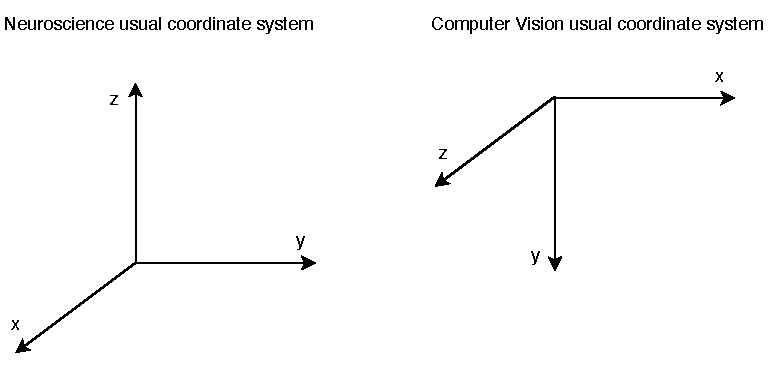
\includegraphics[width=10cm]{images/coordsys.pdf}
	\caption[Neuroscience vs Computer vision usual coordinate systems]{The neuroscience and computer vision 3 dimensional coordinate systems normally used are different; both use the right-hand rule. In Neuroscience, torsion is along the frontal visual x-axis, vertical angles along the inter-aural y-axis, and horizontal angles along the bottom-up z-axis.}
	\label{sec2:fig:coordsys}
\end{figure}

\subsection{Donders' and Listing's laws}

As described in the beginning of this section, the orientation of a freely rotating rigid body can be quantified by a horizontal angle, $\theta$, a vertical angle, $\phi$,  and a torsional angle, $\psi$ (around the z, y and x, axis, respectively), relative to a starting position (the primary direction) for which all three angles are zero. Thus, 3 degrees of freedom.

However, as referred before, Donders' law states that the orientation of the eye, when looking in a specific direction at infinity, is always the same; in other words, as described by Donders: 
"with the head erect and looking at infinity, any gaze direction has a unique torsional angle, regardless the path followed by the eye to get there". Thus, the eye has 2 degrees of freedom for pointing.

Moreover, the 3D orientations of the eye can be uniquely described by head-fixed Cartesian coordinate system of single-axis rotations (section \ref{killme}) that bring the eye from the primary position to the current orientation. Described in this way, Listing's law holds that the rotation axis corresponding to all possible eye orientations are confined to the yz-plane, called Listing's plane, in neuroscience. The primary position of the eye is an unique position 
from which any other eye position can be reached through rotation around an axis lying in Listing's plane. This hypothetical rotation axis is defined by a vector 
$ \mathbf{r}  = \left( r _ { x } , r _ { y } , r _ { z } \right)$, where $r _ { x }$, the torsional component perpendicular to the Listing's plane, is zero. 
Figure \ref{sec2:fig:monkey} illustrates that this law is very precise, by showing 3500 different eye orientations made by a head-restrained monkey, where the left image is the frontal view on the rotation axis, representing the gazed points coordinates of the horizontal, $r_{ y }$, and vertical, $r_{ z }$, components of the axis, and the right-hand plot is a side view, representing the coordinates expressed by the  horizontal and torsional, $r_x$, components. A plane is clearly seen around $r_x = 0$ with little deviation ($\sigma _x \approx 0.6$ deg).
\begin{figure}[ht]
	\centering
	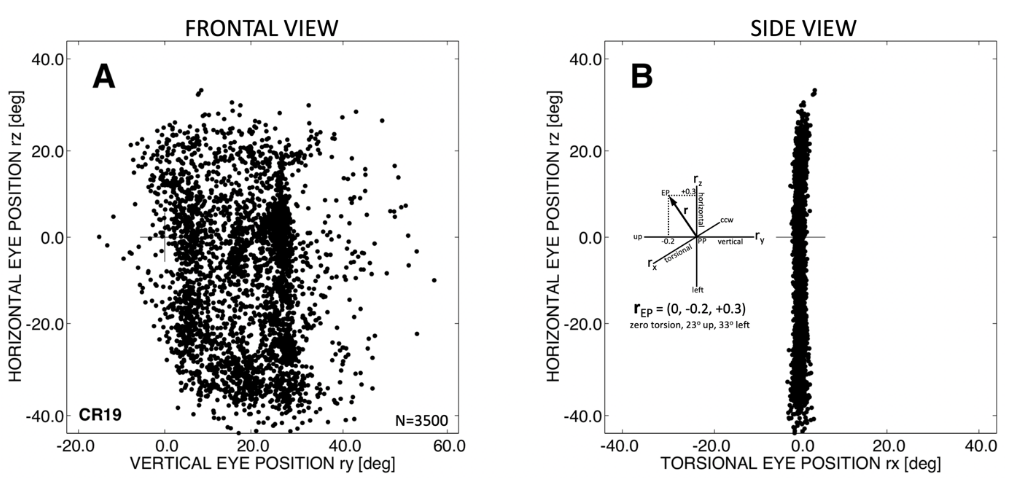
\includegraphics[width=13cm]{images/ll.png}
	\caption[Listing’s law, illustrated for 3500 eye orientations made by a head-restrained monkey]{Listing’s law, illustrated for 3500 eye orientations made by a head-restrained monkey, freely looking around in the laboratory room. Eye fixations are represented by the head-fixed Cartesian components of the 3D rotation axes, expressed in half-radians, and calculated as $angle = 2 \cdot atan(component)$. \cite{donders}}
	\label{sec2:fig:monkey}
\end{figure}

However, if the initial eye position is not the primary position, it should be noted that the dynamic angular velocity axis, $ \mathbf{\omega}$, that rotates the eye from one orientation in the Listing's plane to another, e.g. during a saccadic eye movement, is {\bf not} confined to the plane itself. It will typically have a torsional component, $\omega_x \neq 0$, as it depends on the initial eye position, $ \mathbf{r_1}  = (0, r_{1y}, r_{1z})$ and the saccade difference vector in Listing's Plane, $\mathbf{d_{12} }\equiv \mathbf{r_2} - \mathbf{r_1} = (0, d_{12y},d_{12z})$ that carries the eye to the final eye position, resulting in
\begin{equation}
\omega _x = r_{1y} \cdot d_{12z} - r_{1z} \cdot d_{12y}.
\end{equation} 
This expression can be reached, using the representation on section \ref{killme}, through the following:
\begin{enumerate}
	\item When rotating the eye, on the conditions that assure the existence of Listing's plane, from one position, $\bf r_1$, to another, $\bf r_2$, the resulting rotation axis will be $\bf r_{12} = r_1  \cdot r_2^{-1}$;
	\item A rotation vector can be obtained by
	\begin{equation}
	\mathbf{r _ { 21 } } = \frac { \mathbf{r _ { 2 }} - \mathbf{r _ { 1 } }+ \mathbf{r _ { 1 }} \times \mathbf{r _ { 2 } }} { 1 + \mathbf{r _ { 1 }} \cdot \mathbf{r _ { 2 } }} \approx \mathbf{r _ { 2 }} - \mathbf{r _ { 1 }} + \mathbf{r _ { 1 }} \times \mathbf{r _ { 2 }} \equiv \mathbf{d _ { 12 }} + \mathbf{r _ { 1 } }\times \mathbf{d_{12 }} ,
	\end{equation}
	where $\mathbf{r _ { 1 }} \cdot \mathbf{r _ { 2 }} << 1$ for angles smaller then 30 degrees which is normally the case on eye rotations.
	\item Expanding the previous equation to
	\begin{equation}
	\mathbf{r _ { 21 }} = 
	\left( \begin{array} { c } { 0 } \\ \mathbf{{ d_{12y}}} \\ \mathbf{{d_{12z}}}\end{array}\right) +  \left( \begin{array} { c } { 0 } \\ \mathbf{{ r _ { 1 y } }} \\ \mathbf{{ r _ { 1 z }  }}\end{array}\right) 
	\times \left( \begin{array} { c } { 0 } \\ \mathbf{{ d_{12y}}} \\ \mathbf{{ d_{12z} }}  \end{array} \right),
	\end{equation}
	$\bf r_{12x} = r_{1y} \cdot d_{12z} - r_{1z} \cdot d_{12y}$ is obtained and corresponds to the angular velocity component $\bf \omega_x$.
\end{enumerate}
\cite{donders} \cite{eye}